\documentclass[11pt,a4paper]{article}

% ── Packages ────────────────────────────────────────────────────────
\usepackage[utf8]{inputenc}
\usepackage[T1]{fontenc}
\usepackage{lmodern}
\usepackage{amsmath,amssymb,amsfonts}
\usepackage{graphicx}
\usepackage{booktabs}
\usepackage{xcolor}
\usepackage{hyperref}
\usepackage[margin=2.5cm]{geometry}
\usepackage{enumitem}
\usepackage{caption}
\usepackage{float}

\hypersetup{
    colorlinks=true,
    linkcolor=blue!70!black,
    citecolor=blue!70!black,
    urlcolor=blue!70!black,
}

% ── Title ───────────────────────────────────────────────────────────
\title{Bounded Geometric Phase Transition in Finite Causal Posets\\with Exact Entropy}
\author{Gang Zhang}
\date{}

% ════════════════════════════════════════════════════════════════════
\begin{document}
\maketitle

% ── Abstract ────────────────────────────────────────────────────────
\begin{abstract}
The Kleitman--Rothschild (KR) theorem implies that generic finite posets are 3-layered and maximally entropic, posing a fundamental obstacle to geometric phase emergence in discrete causal models. We construct a 7-family poset ensemble and compute exact linear extension counts for $N = 10$--$44$ elements to study action-weighted competition between Lorentzian-like geometric structures and KR-type high-entropy posets. Under a decomposable action combining neutral and geometric penalty terms, we find that the critical geometric coupling $\gamma_c$ remains $O(1)$ across all tested sizes --- the first finite-size evidence of a bounded phase transition threshold in this setting. Systematic ablation of seven geometric sub-terms identifies a minimal backbone of two constraints: global layer-shape balance and dimensional scale consistency. Crucially, the latter can be replaced by a non-target-anchored variant (penalizing local--global dimension inconsistency rather than deviation from a specific $d = 2$ target), with $\gamma_c$ preserved at the same order of magnitude. These results provide finite-size evidence that Lorentzian-like order in discrete causal structures can emerge from structural self-consistency constraints, without requiring dimension-specific priors.
\end{abstract}

% ── 1. Introduction ─────────────────────────────────────────────────
\section{Introduction}

The hypothesis that spacetime is fundamentally discrete --- a locally finite partial order (poset) whose elements are causally related events --- lies at the heart of causal set theory (CST)~\cite{bombelli1987,sorkin2005}. A central challenge for this program is the \emph{entropy catastrophe}: the Kleitman--Rothschild (KR) theorem~\cite{kleitman1975} establishes that, asymptotically, almost all labeled finite posets consist of three layers with bipartite random connectivity and maximal linear extension count. If one weights posets by the pure combinatorial entropy $H = \log(\text{number of linear extensions})$, the partition function is overwhelmingly dominated by these non-geometric, KR-type structures. Geometric order --- the kind of layered, causally propagating structure that would correspond to a Lorentzian manifold under coarse-graining --- occupies an exponentially small fraction of the configuration space.

Several strategies have been proposed to address this. The Benincasa--Dowker (BD) action~\cite{benincasa2010,benincasa2011} provides a discrete analogue of the Einstein--Hilbert action on causal sets, with a well-defined continuum limit; in 2D, numerical work has found evidence for phase-transition-like behavior and finite-size scaling in BD-based causal set quantum gravity models~\cite{surya2012,glaser2018}, with related developments in dimensionally restricted settings~\cite{cunningham2020}. Separately, Loomis and Carlip~\cite{loomis2018} gave an analytic argument for suppression of a large class of non-manifold-like causal sets (notably two-level orders) in a Lorentzian path integral with Einstein--Hilbert weighting. Carlip~\cite{carlip2017} and Surya~\cite{surya2019} provide broad reviews of dimensional reduction and causal set quantum gravity, including discussions of entropy challenges in causal set path sums (see also Henson~\cite{henson2006} and Dowker~\cite{dowker2005}). At a more combinatorial level, phase transitions in random partial orders have been studied since Dhar~\cite{dhar1978} and Pr{\"o}mel--Steger--Taraz~\cite{promel2001}. However, explicit finite-$N$ KR-versus-geometric competition curves computed with exact linear-extension entropy remain scarce; here we provide a direct $\gamma_c(N)$ scan with exact entropy in the confirmatory window $N=10$--$44$.

In this work, we take a direct numerical approach. We construct an ensemble of seven structurally distinct poset families, compute exact linear extension counts using dynamic programming for $N$ up to 44, and define a decomposable action with separately controllable neutral and geometric penalty terms. Our main finding is that the critical coupling $\gamma_c$ for Lorentzian-like 2D posets to overtake KR posets remains bounded and $O(1)$ across all tested sizes.

To address the natural concern that this result might be circular --- that geometric penalties simply ``reward looking geometric'' --- we perform a systematic ablation study. We identify which of seven geometric sub-terms are necessary for the phase transition and which are dispensable. The two critical drivers are (i)~a global layer-shape constraint that penalizes degenerate causal chain depth, and (ii)~a dimensional proxy. We then replace the latter with a \emph{non-target-anchored} alternative that penalizes local--global dimension inconsistency without specifying any target dimension. The phase transition survives this replacement, establishing that the mechanism does not require a dimension-specific prior.

% ── 2. Framework ────────────────────────────────────────────────────
\section{Framework}

\subsection{Poset Ensemble}

We consider finite posets $P = (V, \leq)$ with $|V| = N$ elements. Each poset is represented by its transitive reduction (Hasse diagram). We generate samples from seven structurally distinct families:

\begin{itemize}[nosep]
    \item \textbf{Lorentzian-like 2D} (\texttt{lor2d}): Layered posets mimicking 2D causal diamond structure, with layer sizes following a diamond profile and inter-layer edges determined by spatial proximity.
    \item \textbf{Lorentzian-like 3D} (\texttt{lor3d}): Three-dimensional analogue with broader layers and correspondingly lower comparable fraction.
    \item \textbf{KR-like} (\texttt{kr}): Three-layer bipartite posets with random inter-layer edges, approximating the KR structure that dominates the entropy landscape.
    \item \textbf{Multi-layer random} (\texttt{mlr}): Random layered posets with uniformly drawn layer count and random inter-layer connectivity.
    \item \textbf{Transitive percolation} (\texttt{tp}): Posets generated by transitive closure of a random DAG on a totally ordered set with independent edge probability.
    \item \textbf{Interval order} (\texttt{int}): Posets arising from random intervals on the real line, where $x < y$ iff the interval of $x$ lies entirely below that of $y$.
    \item \textbf{Absolute layered} (\texttt{abs}): Fully connected layered posets with all inter-layer edges present.
\end{itemize}

For each family and each $N \in \{10, 12, 14, 16, 20, 24, 28, 32, 36, 40, 44\}$, we generate $K = 5$ independent samples. We distinguish two sample sets: a \textbf{confirmatory mainline} (used in Section~\ref{sec:bounded} for the primary $\gamma_c$ curve) and an independent \textbf{exploratory set} (used in Sections~\ref{sec:ablation}--\ref{sec:replacement} for ablation and replacement studies). Both sets use the same generators and parameters; they differ only in random seeds. The $A_2$ baseline $\gamma_c$ values are $O(1)$ in both sets, ensuring that qualitative conclusions are robust to sample variation.

\subsection{Exact Linear Extension Count}

The entropy of a poset $P$ is defined as $H(P) = \log |L(P)|$, where $L(P)$ is the set of linear extensions (topological sorts). We compute $|L(P)|$ exactly using dynamic programming over antichains~\cite{brightwell1991}. The state space is the set of all antichains of the poset (equivalently characterized as maximal antichains of the remaining down-set); transitions correspond to removing a minimal element.

We emphasize that $\log|L(P)|$ is used here as a \emph{combinatorial measure term}: for an unlabeled poset $P$, the number of natural labelings consistent with the order is exactly the number of linear extensions, so a labeled path sum (or any proxy that samples labelings rather than isomorphism classes) implicitly weights $P$ by $|L(P)|$. For discussions of entropy factors in causal set path sums and their competition with action terms, see e.g.~\cite{mathur2021}.

This is a choice of ensemble and measure, not a claim that $\log|L(P)|$ is a
unique or physically correct definition of gravitational entropy. Alternative
formulations can sum over \emph{unlabeled} posets and divide by automorphism
factors (e.g.\ $1/|\mathrm{Aut}(P)|$), which changes the effective entropy term
and may change which families dominate. Here we focus on the labeled (or
label-sampling) setting in which linear extensions appear as the natural
combinatorial measure factor.

A key structural observation is that the computational cost of this algorithm depends strongly on the poset's antichain structure. For \texttt{lor2d}, whose antichain width grows slowly with $N$, exact computation remains sub-second to $N = 48$. For \texttt{kr}, whose middle layer is $O(N)$, the cost grows dramatically and becomes impractical beyond $N \approx 50$. This asymmetry is a structural fact about the posets, not an algorithmic artifact.

\begin{table}[H]
\centering
\caption{Exact linear extension computation time.}
\label{tab:timing}
\begin{tabular}{ccc}
\toprule
$N$ & \texttt{lor2d} time & \texttt{kr} time \\
\midrule
30 & 0.02\,s & 0.31\,s \\
40 & 0.07\,s & 14.3\,s \\
44 & 0.09\,s & 54.0\,s \\
\bottomrule
\end{tabular}
\end{table}

\subsection{Action Definition}

We define three action paths to separate neutral and geometric contributions:
\begin{align}
    A_1 &= -\beta H + \gamma \cdot I_{\text{neutral}} \label{eq:A1} \\
    A_2 &= -\beta H + \gamma \cdot (I_{\text{neutral}} + I_{\text{geometric}}) \label{eq:A2} \\
    A_3 &= -\beta H + \gamma \cdot I_{\text{geometric}} \label{eq:A3}
\end{align}
where $\beta = 1$ throughout, and $\gamma$ is the geometric coupling constant.

The \textbf{neutral penalty} $I_{\text{neutral}}$ comprises terms that do not reference any specific geometric structure: comparable fraction deviation, degree variance, and layer entropy.

The \textbf{geometric penalty} $I_{\text{geometric}}$ is decomposed into seven sub-terms:

\begin{table}[H]
\centering
\caption{Geometric sub-terms and their physical motivations.}
\label{tab:subterms}
\begin{tabular}{lll}
\toprule
Sub-term & Symbol & Physical motivation \\
\midrule
Width-height balance & $g_{\text{wh}}$ & Penalizes degenerate causal depth (width $\gg$ height) \\
Dimension proxy & $g_{\text{dim}}$ & Penalizes deviation from effective dimension target \\
Interval shape & $g_{\text{int}}$ & Penalizes non-diamond-shaped causal intervals \\
Comparability window & $g_{\text{cmp}}$ & Penalizes extreme comparable fraction \\
Cover density & $g_{\text{cov}}$ & Penalizes sparse/dense covering relations \\
Interval profile & $g_{\text{prf}}$ & Penalizes irregular interval size distribution \\
Layer smoothness & $g_{\text{lyr}}$ & Penalizes irregular layer size variation \\
\bottomrule
\end{tabular}
\end{table}

Each sub-term is normalized to $[0, 1]$ per poset.

\subsection{Phase Transition Criterion}

For each $N$, we compute the mean action scores $\bar{S}_{\text{lor2d}}(\gamma)$ and $\bar{S}_{\text{kr}}(\gamma)$ across samples. The critical coupling is defined as:
\begin{equation}
    \gamma_c(N) = \inf\bigl\{\gamma > 0 : \bar{S}_{\text{lor2d}}(\gamma) < \bar{S}_{\text{kr}}(\gamma)\bigr\}
    \label{eq:gamma_c}
\end{equation}
If $\gamma_c$ exists and remains bounded as $N$ increases, this constitutes evidence for a geometric phase transition.

% ── 3. Results ──────────────────────────────────────────────────────
\section{Results}

\subsection{Bounded $\gamma_c$ Under $A_2$}
\label{sec:bounded}

Under the full action $A_2$, $\gamma_c$ exists for all tested $N$ and remains $O(1)$:

\begin{table}[H]
\centering
\caption{Critical coupling $\gamma_c$ under $A_2$ (confirmatory mainline, exact entropy).}
\label{tab:gamma_c}
\begin{tabular}{cccccccccccc}
\toprule
$N$ & 10 & 12 & 14 & 16 & 20 & 24 & 28 & 32 & 36 & 40 & 44 \\
\midrule
$\gamma_c$ & 9.19 & 0.74 & 0.78 & 0.69 & 0.15 & 0.26 & 1.00 & 0.69 & 0.57 & 0.25 & 0.15 \\
\bottomrule
\end{tabular}
\end{table}

The $N = 10$ value is an outlier due to finite-size effects in the small-poset regime. For $N \geq 12$, all values lie within $[0.15, 1.00]$ (Figure~\ref{fig:gamma_c}).

\begin{figure}[htbp]
    \centering
    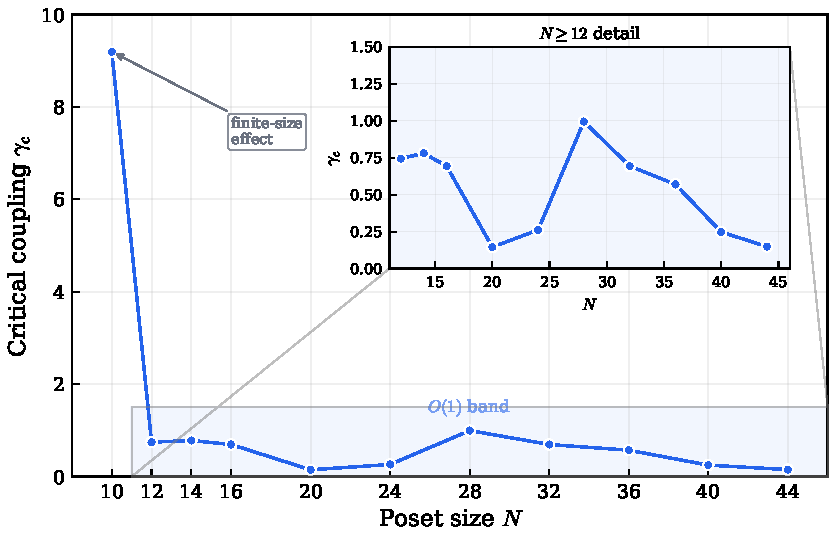
\includegraphics[width=0.85\textwidth]{manuscript_figures/fig1_gamma_c_curve.pdf}
    \caption{Critical coupling $\gamma_c(N)$ under $A_2$ (exact entropy) for Lor2D vs KR. The $N=10$ outlier reflects finite-size effects; for $N \geq 12$, $\gamma_c$ remains $O(1)$ within $[0.15, 1.00]$. Inset shows the $N \geq 12$ detail.}
    \label{fig:gamma_c}
\end{figure}

\textbf{Critical control}: Under $A_1$ (neutral penalty only), no $\gamma_c$ exists at any tested $N$ (verified across $N = 20$--$44$ in the ablation set and $N = 10$--$16$ in the confirmatory set). Lorentzian-like structures never overtake KR without geometric penalties. This supports the conclusion that the phase transition is driven by the geometry--entropy competition encoded in $A_2$, not by neutral structural differences alone.

\subsection{Ablation of Geometric Sub-Terms}
\label{sec:ablation}

We systematically remove each of the seven geometric sub-terms from $A_2$ and re-compute $\gamma_c$:

\begin{table}[H]
\centering
\caption{Single-term ablation results ($N = 20$--$44$, exploratory set).}
\label{tab:ablation}
\begin{tabular}{lll}
\toprule
Removed sub-term & $\gamma_c$ at $N=20$--$44$ & Role \\
\midrule
None (full $A_2$) & Exists at all $N$ & Baseline \\
$g_{\text{wh}}$ (width-height) & Fails from $N \geq 36$ & \textbf{Critical} \\
$g_{\text{dim}}$ (dimension proxy) & Fails at $N = 36, 44$ & \textbf{Critical} \\
$g_{\text{int}}$ (interval shape) & All $N$, shifted higher & Enhancer \\
$g_{\text{cmp}}$ (comparability) & All $N$ & Non-critical \\
$g_{\text{cov}}$ (cover density) & All $N$ & Non-critical \\
$g_{\text{prf}}$ (interval profile) & All $N$ & Non-critical \\
$g_{\text{lyr}}$ (layer smoothness) & All $N$ & Non-critical \\
\bottomrule
\end{tabular}
\end{table}

\textbf{Combined ablation}: Removing both critical drivers ($g_{\text{wh}}$ and $g_{\text{dim}}$) simultaneously causes $\gamma_c$ to vanish at all $N$. Retaining only interval-type terms ($g_{\text{int}} + g_{\text{prf}}$) also fails to produce any phase transition. Conversely, removing all interval terms while keeping the two critical drivers preserves $\gamma_c$ at all $N$ (with a modest upward shift).

This establishes a clear \textbf{backbone--shell structure} (Figure~\ref{fig:ablation}):
\begin{itemize}[nosep]
    \item \textbf{Backbone} (necessary): $g_{\text{wh}} + g_{\text{dim}}$
    \item \textbf{Shell} (enhancing but not necessary): all other sub-terms
\end{itemize}

\begin{figure}[htbp]
    \centering
    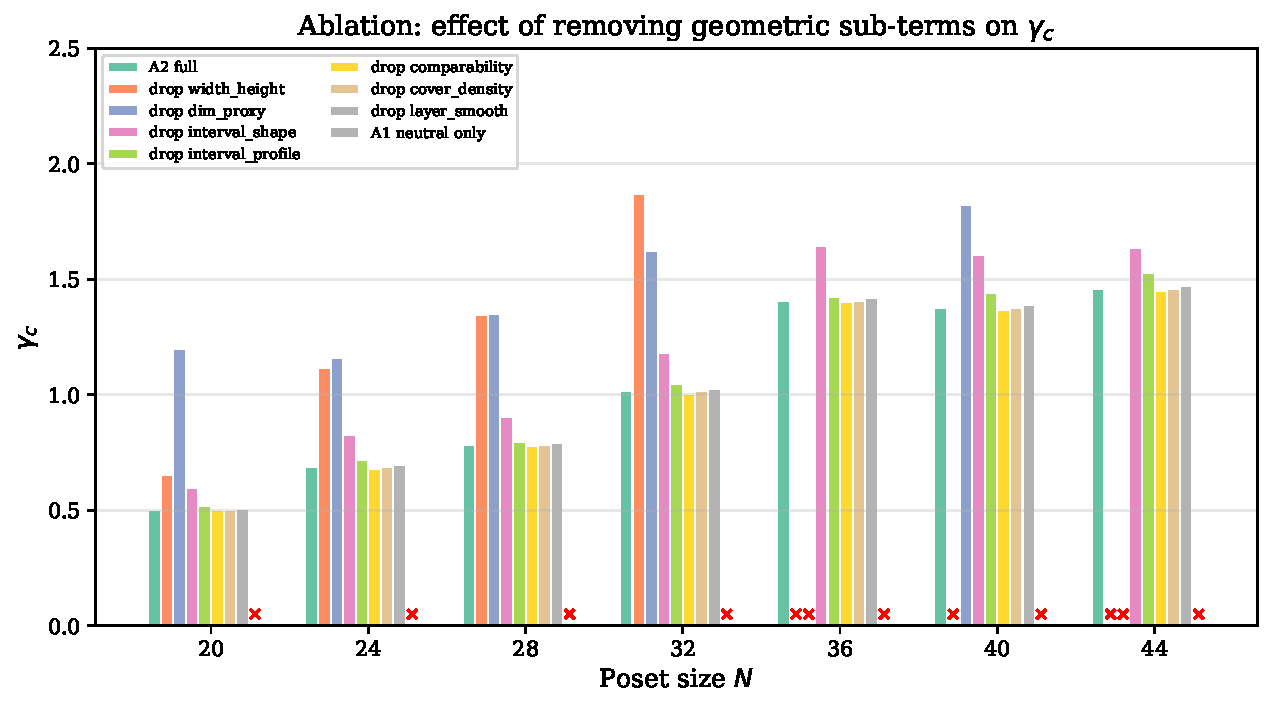
\includegraphics[width=0.95\textwidth]{manuscript_figures/fig2_ablation_summary.pdf}
    \caption{Ablation summary --- $\gamma_c$ under the full action and with each sub-term removed, for $N = 20$--$44$. Dashes indicate absent phase transitions (no crossing). Red-bordered rows mark the two critical sub-terms. Only width-height balance and dimension proxy are necessary for the phase transition.}
    \label{fig:ablation}
\end{figure}

\subsection{Non-Circular Replacement}
\label{sec:replacement}

The dimension proxy $g_{\text{dim}}$ penalizes deviation from a target dimension $d = 2$. Since our test target is a 2D structure, this raises a circularity concern.

We construct a replacement term, $g_{\text{con}}$ (\textbf{dimension consistency}), which penalizes inconsistency between local interval-estimated dimensions and the global dimension, without specifying any target value. Formally:
\begin{equation}
    g_{\text{con}}(P) = \text{Var}[d_{\text{local}}] + \bigl(\overline{d}_{\text{local}} - d_{\text{global}}\bigr)^2
    \label{eq:gcon}
\end{equation}
where $d_{\text{local}}(x,y)$ is the order-fraction dimension proxy applied to sampled causal intervals $I(x,y) = \{z : x < z < y\}$ with $|I| \geq 4$, $d_{\text{global}}$ is the same estimator applied to the full poset, and the dimension proxy is $d_{\text{eff}}(r) = 2 + 6(R_{2,\text{ref}} - r)$ with $R_{2,\text{ref}} = 0.5009$ being the 2D Minkowski order fraction. Note that while the \emph{estimator's} calibration point references 2D, the \emph{penalty} $g_{\text{con}}$ does not penalize any specific dimension --- it penalizes dimensional \emph{inconsistency} across scales.

\begin{table}[H]
\centering
\caption{Non-circular replacement results (exploratory set).}
\label{tab:replacement}
\begin{tabular}{lcc}
\toprule
Configuration & $N = 20$--$40$ & $N = 44$ \\
\midrule
$A_2$ full (original) & \checkmark & \checkmark \\
Replace $g_{\text{dim}} \to g_{\text{con}}$ & \checkmark & \checkmark \\
$g_{\text{wh}} + g_{\text{con}}$ only & \checkmark & $\times$ (weight $1.0\times$) \\
$g_{\text{wh}} + g_{\text{con}}$ only & \checkmark & \checkmark (weight $1.3\times$)$^*$ \\
$g_{\text{wh}}$ only & $N=24,28$ only & $\times$ \\
\bottomrule
\end{tabular}
\begin{flushleft}
\small $^*$Weight scan experiment; data not included in the released exploratory CSV.
\end{flushleft}
\end{table}

The replacement preserves $\gamma_c$ at the same order of magnitude across all $N = 20$--$44$ (Figure~\ref{fig:replacement}). The minimal non-circular backbone ($g_{\text{wh}} + g_{\text{con}}$) covers $N = 20$--$40$ with matched weights and extends to $N = 44$ with a modest 30\% weight increase.

\begin{figure}[htbp]
    \centering
    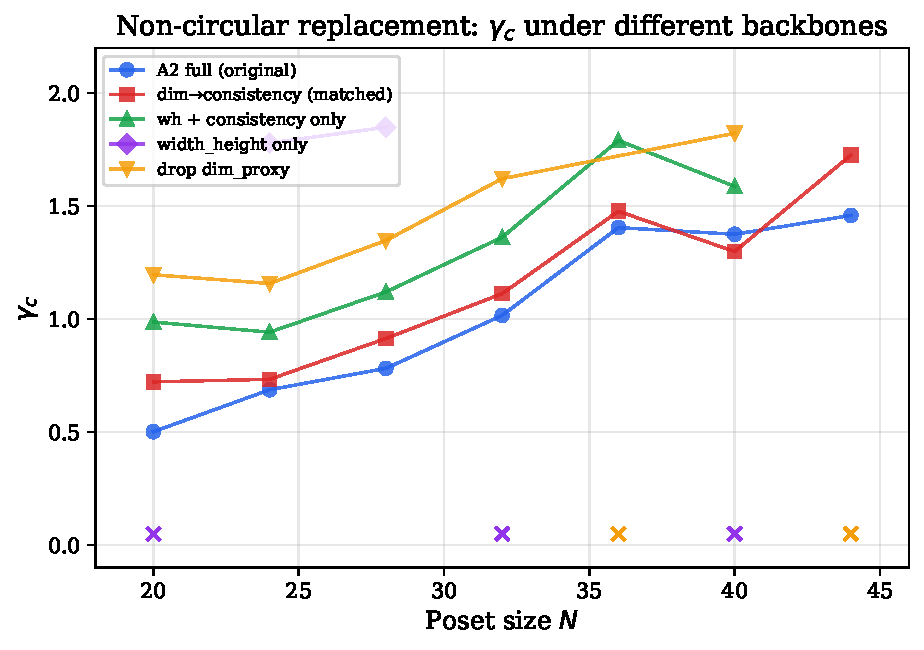
\includegraphics[width=0.85\textwidth]{manuscript_figures/fig3_noncircular_replacement.pdf}
    \caption{Non-circular replacement comparison --- $\gamma_c$ under original $A_2$, scale-matched consistency replacement, and reduced backbones. $\times$ marks indicate absent crossings.}
    \label{fig:replacement}
\end{figure}

This demonstrates that the phase transition mechanism does not require a target-dimension prior. The essential information is:
\begin{enumerate}[nosep]
    \item \textbf{Causal chain non-degeneracy} (width-height balance): independent of dimension.
    \item \textbf{Dimensional scale consistency} (local--global coherence): structurally motivated, dimension-agnostic.
\end{enumerate}

% ── 4. Discussion ───────────────────────────────────────────────────
\section{Discussion}

\subsection{Interpretation}

Our results provide the first finite-size evidence for a bounded geometric phase transition in poset ensembles with exact entropy computation. The key insight from the ablation analysis is that the mechanism driving geometric dominance can be reduced to two structurally interpretable constraints, neither of which requires specifying a target spacetime dimension.

The width-height balance constraint has a particularly clean physical interpretation: in any causal structure, the ratio of spatial extent (antichain width) to temporal extent (longest chain) characterizes the degree of causal propagation. KR posets, with their 3-layer structure and $O(N)$ middle layer, represent maximally degenerate causal chains. Penalizing this degeneracy is not equivalent to ``rewarding Lorentzian geometry'' --- it is equivalent to requiring that the causal order supports non-trivial temporal evolution.

The dimension consistency constraint captures the idea that genuine manifold-like structures should exhibit coherent dimensionality across scales. Lorentzian-like posets naturally satisfy this; KR posets do not. The fact that this constraint need not specify $d = 2$ is important: it means the mechanism would, in principle, favor \emph{any} dimensionally coherent geometric structure over KR, not specifically 2D ones.

\subsection{Relation to Prior Work}

Carlip~\cite{carlip2017} reviews the broader landscape of dimensional
reduction in quantum gravity, including causal set approaches and the challenge
posed by high-entropy non-manifold-like orders. Our work contributes a concrete
finite-$N$ computation of $\gamma_c(N)$ with exact linear-extension measure
factors and systematic ablation, aimed at diagnosing which structural
constraints can overcome KR dominance in a labeled (or label-sampling) setting.

Loomis and Carlip~\cite{loomis2018} analytically demonstrated the suppression of non-manifold-like sets in the causal set path integral; Surya~\cite{surya2012} and Cunningham and Surya~\cite{cunningham2020} studied CST partition functions in dimensionally restricted settings. Our approach is complementary: rather than sampling from the full space of $N$-element posets, we compare representative structures from distinct families, which allows exact computation and complete ablation control. Glaser~\cite{glaser2018} studied finite-size scaling in 2D CST, finding evidence for a continuum phase; our finite-size evidence for bounded $\gamma_c$ is consistent with and complementary to that work.

\textbf{Relation to the Benincasa--Dowker action.} The standard discrete action in CST is the Benincasa--Dowker (BD) action~\cite{benincasa2010,benincasa2011}, which provides a direct discretization of the Einstein--Hilbert action with a known continuum limit. Our action $A_2$ differs from the BD action in both form and purpose: $A_2$ is constructed as a decomposable penalty functional for ablation studies, with each sub-term targeting a specific structural property. It is not a discretization of any known continuum action and does not have a known continuum limit. The advantage of our approach is that the decomposable structure allows systematic ablation to identify which structural constraints drive geometric phase emergence --- a diagnostic capability that the BD action, as a single composite quantity, does not directly provide. Whether the BD action itself produces a bounded $\gamma_c$ in the sense defined here is an important open question for future work.

\subsection{Limitations}

Several important caveats apply:

\begin{enumerate}[nosep]
    \item \textbf{Finite size}: $N = 44$ is far from any thermodynamic limit. Whether $\gamma_c$ remains bounded as $N \to \infty$ is the central open question.
    \item \textbf{Family coverage}: Seven families do not exhaust all posets. Our claim is ``competitive phase among tested structural types,'' not global dominance.
    \item \textbf{Generator dependence}: Each family is defined by a specific generator. Structural properties (and thus penalty values) depend on generator parameters.
    \item \textbf{Weight sensitivity}: The minimal non-circular backbone requires weight adjustment at $N = 44$, suggesting proximity to a critical boundary at larger~$N$.
    \item \textbf{Estimator calibration}: The dimension proxy $d_{\text{eff}}(r)$ is calibrated at the 2D Minkowski order fraction $R_{2,\text{ref}} = 0.5009$. While the consistency penalty $g_{\text{con}}$ does not penalize deviation from $d = 2$, the estimator's calibration point introduces a residual 2D reference. A fully dimension-agnostic estimator (e.g., based on interval cardinality ratios without a fixed reference) would further strengthen the non-circularity claim.
\end{enumerate}

\subsection{Outlook}

The most important next step is pushing the exact computation to larger $N$. The favorable scaling of exact linear extension counts for Lorentzian-like posets (sub-second to $N = 48$) makes this feasible for the geometric side; the bottleneck is KR computation. Beyond exact computation, an independent verification using Markov chain methods on the full poset space at moderate $N$ would significantly strengthen the case.

The non-circular replacement result also opens a conceptual direction: if the minimal requirements for geometric phase emergence are causal chain non-degeneracy and dimensional scale consistency, then these two properties may serve as order parameters for detecting geometric phases in more general discrete quantum gravity models.

% ── References ──────────────────────────────────────────────────────
\begin{thebibliography}{20}

\bibitem{bombelli1987}
L.~Bombelli, J.~Lee, D.~Meyer, and R.~D.~Sorkin,
``Space-time as a causal set,''
\textit{Phys.\ Rev.\ Lett.} \textbf{59}, 521 (1987).

\bibitem{sorkin2005}
R.~D.~Sorkin,
``Causal sets: Discrete gravity,''
in \textit{Lectures on Quantum Gravity}, ed.\ A.~Gomberoff and D.~Marolf
(Springer, 2005). arXiv:gr-qc/0309009.

\bibitem{kleitman1975}
D.~J.~Kleitman and B.~L.~Rothschild,
``Asymptotic enumeration of partial orders on a finite set,''
\textit{Trans.\ Amer.\ Math.\ Soc.} \textbf{205}, 205--220 (1975).

\bibitem{carlip2017}
S.~Carlip,
``Dimension and dimensional reduction in quantum gravity,''
\textit{Class.\ Quantum Grav.} \textbf{34}, 193001 (2017).
arXiv:1705.05417. DOI:~10.1088/1361-6382/aa8535.

\bibitem{surya2019}
S.~Surya,
``The causal set approach to quantum gravity,''
\textit{Living Rev.\ Relativ.} \textbf{22}, 5 (2019).
arXiv:1903.11544. DOI:~10.1007/s41114-019-0023-1.

\bibitem{loomis2018}
S.~P.~Loomis and S.~Carlip,
``Suppression of non-manifold-like sets in the causal set path integral,''
\textit{Class.\ Quantum Grav.} \textbf{35}, 024002 (2018).
DOI:~10.1088/1361-6382/aa980b.

\bibitem{dhar1978}
D.~Dhar,
``Entropy and phase transitions in partially ordered sets,''
\textit{J.\ Math.\ Phys.} \textbf{19}, 171 (1978).

\bibitem{promel2001}
H.~J.~Pr{\"o}mel, A.~Steger, and A.~Taraz,
``Phase transitions in the evolution of partial orders,''
\textit{J.\ Comb.\ Theory Ser.\ A} \textbf{94}, 230 (2001).

\bibitem{brightwell1991}
G.~Brightwell and P.~Winkler,
``Counting linear extensions,''
\textit{Order} \textbf{8}, 225--242 (1991).

\bibitem{mathur2021}
S.~Mathur, J.~S.~Singh, and S.~Surya,
``Entropy and the link action in causal set path sums,''
arXiv:2009.07232.

\bibitem{cunningham2020}
W.~J.~Cunningham and S.~Surya,
``Dimensionally restricted causal set quantum gravity: Examples in two and three dimensions,''
\textit{Class.\ Quantum Grav.} \textbf{37}, 054002 (2020).
arXiv:1908.11647. DOI:~10.1088/1361-6382/ab60b7.

\bibitem{benincasa2010}
D.~M.~T.~Benincasa and F.~Dowker,
``The scalar curvature of a causal set,''
\textit{Phys.\ Rev.\ Lett.} \textbf{104}, 181301 (2010).
arXiv:0911.2725. DOI:~10.1103/PhysRevLett.104.181301.

\bibitem{benincasa2011}
D.~M.~T.~Benincasa, F.~Dowker, and B.~Schmitzer,
``The random discrete action for two-dimensional spacetime,''
\textit{Class.\ Quantum Grav.} \textbf{28}, 105018 (2011).
arXiv:1011.5191. DOI:~10.1088/0264-9381/28/10/105018.

\bibitem{rideout2000}
D.~P.~Rideout and R.~D.~Sorkin,
``A classical sequential growth dynamics for causal sets,''
\textit{Phys.\ Rev.\ D} \textbf{61}, 024002 (2000).
arXiv:gr-qc/9904062. DOI:~10.1103/PhysRevD.61.024002.

\bibitem{henson2006}
J.~Henson,
``The causal set approach to quantum gravity,''
in \textit{Approaches to Quantum Gravity}, ed.\ D.~Oriti
(Cambridge University Press, 2009). arXiv:gr-qc/0601121.

\bibitem{dowker2005}
F.~Dowker,
``Causal sets and the deep structure of spacetime,''
in \textit{100 Years of Relativity}, ed.\ A.~Ashtekar
(World Scientific, 2005). arXiv:gr-qc/0508109.

\bibitem{surya2012}
S.~Surya,
``Evidence for the continuum in 2D causal set quantum gravity,''
\textit{Class.\ Quantum Grav.} \textbf{29}, 132001 (2012).
arXiv:1110.6244. DOI:~10.1088/0264-9381/29/13/132001.

\bibitem{glaser2018}
L.~Glaser,
``Finite size scaling in 2d causal set quantum gravity,''
\textit{Class.\ Quantum Grav.} \textbf{35}, 045002 (2018).
arXiv:1706.06432. DOI:~10.1088/1361-6382/aa9540.

\bibitem{glaser2014}
L.~Glaser and S.~Surya,
``Towards a definition of locality in a manifoldlike causal set,''
\textit{Phys.\ Rev.\ D} \textbf{88}, 124026 (2013).
arXiv:1309.3403. DOI:~10.1103/PhysRevD.88.124026.

\end{thebibliography}

% ── Acknowledgments ─────────────────────────────────────────────────
\section*{Acknowledgments}

\textbf{AI Assistance Statement}: This work was conducted in collaboration with large language model assistants (Claude, Anthropic). The AI contributed to experimental design, Python code implementation, data analysis, theoretical interpretation, and manuscript drafting. All scientific decisions, theoretical motivations, and final interpretations were made by the human author, who takes full responsibility for the content. The complete codebase is publicly available at \url{https://github.com/unicome37/poset_phase} for independent verification and reproduction.

\section*{Code and Data Availability}

All code, configuration files, and output data are available at: \url{https://github.com/unicome37/poset_phase}

Archived version with DOI: \url{https://doi.org/10.5281/zenodo.18963421}

\end{document}
